
\begin{frame}{The proposed multiresolution data model (MTSMS)}

  The \acro{MTSMS} model is an storage solution for a time series
  where, in short, the information is spread in different time
  resolutions.

  \vfill

  \begin{enumerate}

  \item Buffer $B=(S,\tau,\delta,f)$. Regularises the time series.
    \begin{itemize}
    \item $\delta$ duration of the consolidation step
    \item $\tau$ last consolidation time
    \item $f$ attribute aggregate function 
    %\item \emph{add}%: $B \times m \mapsto B'$.
    \item \emph{consolidate} buffered S%: $B \mapsto B' \times m'$.
    \end{itemize}

  \item Disc $D=(S,k)$. Finite container.
    \begin{itemize}
    \item Storage bounded: $|S| \leq k$ 
    \item \emph{add} discarding oldest measure %: $D \times m \mapsto D'$
    \end{itemize}

  \item Resolution disc $R=(B,D)$. 
    \begin{itemize}
    \item \emph{add} to buffer%: $(B,D) \times m \mapsto (B',D)$
    \item \emph{consolidate} from buffer to disc%: $(B,D) \mapsto (B',D')$
    \end{itemize}

  \end{enumerate}

  \begin{textblock*}{50mm}(70mm,-44mm)

    \centering

    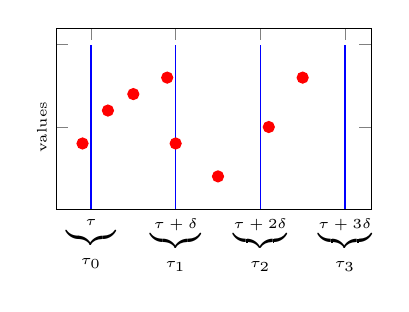
\begin{tikzpicture}
    \begin{axis}[
        width=4cm,
        scale only axis, height=2.3cm,
        ymin = 0,
        yticklabels= {,,\tiny values},
        y tick label style = {rotate=90,anchor=south},
        x tick label style = {font=\tiny},        
        xticklabels={$\underbrace{\tau_{}}_{\tau_0}$,$\underbrace{\tau_0+\delta}_{\tau_1}$,$\underbrace{\tau_{}}_{\tau_0}$,$\underbrace{\tau+\delta}_{\tau_1}$,$\underbrace{\tau+2\delta}_{\tau_2}$,$\underbrace{\tau+3\delta}_{\tau_3}$},
        ]
 
    \addplot[ycomb,blue] coordinates {
        (20,10)
        (30,10)
        (40,10)
        (50,10)
    }; 

    \addplot[red,only marks, mark = *] coordinates {
        (19,4)
        (22,6)
        (25,7)
        (29,8)
        (30,4)
        (35,2)
        (41,5)
        (45,8)
    };

  \end{axis}
  \end{tikzpicture}


  $f: S \times [\tau,\tau+\delta] \mapsto m'$


   \end{textblock*}

\end{frame}




\begin{frame}{Multiresolution model: architecture}

  \begin{enumerate}
    \setcounter{enumi}{3}
  \item Multiresolution database $M=\{R_0,\ldots,R_d \}$. 
    \begin{itemize}
    \item Each \acro{MTSMS} database contains only one time series.
    \item Time series is stored regularised
    \item Time series is distributed with different resolutions
    \end{itemize}
  \end{enumerate}



  \begin{center}
    \begin{tikzpicture}
 \tikzset{
        myarrow/.style={->, >=latex',  thick},
      }
      

  \node[rectangle,draw,minimum height=6cm,minimum width=9cm] (m) {};
  \draw[shift=( m.south west)]   
  node[above right] {base de dades multiresolució};


  %discmig
  \node (m.center) (discr1) {...};

  %discr
  
  \node[ellipse,draw,minimum height=3.5cm,minimum width=2.5cm,alias=discr0] [left=of discr1] {};
  \node[above=0cm of discr0.north] {R0};
  \node[below=0cm of discr0] {disc resolució};

  \node[cylinder, draw, shape border rotate=90, aspect=0.25,alias=buffer0] [below=3mm of discr0.north] {buffer};
  \node[circle, draw,alias=disc0]  [above=3mm of discr0.south] {disc} ;
  \draw [->] (disc0.center)++(.4:.4cm) arc(0:180:.4cm);
  \draw[myarrow] (buffer0.bottom) -- (disc0.north);


  %discrd

  \node[ellipse,draw,minimum height=3.5cm,minimum width=2.5cm,alias=discrd] [right=of discr1] {};
  \node[above=0cm of discrd] {Rd};
  \node[below=0cm of discrd] {disc resolució};

  \node[cylinder, draw, shape border rotate=90, aspect=0.25,alias=bufferd] [below=3mm of discrd.north] {buffer};
  \node[circle, draw,alias=discd]  [above=3mm of discrd.south] {disc} ;
  \draw [->] (discd.center)++(.4:.4cm) arc(0:180:.4cm);
  \draw[myarrow] (bufferd.bottom) -- (discd.north);



  %mesura 
  \node[above=1cm of m.north] (m0) {};

  \draw[myarrow] (m0) -- (m.north) 
  node[right,midway] {mesura};

  \draw[myarrow] (m.north) -- (buffer0);
  \draw[myarrow] (m.north) -- (bufferd);
  \draw[myarrow] (m.north) -- (discr1);

\end{tikzpicture}
  \end{center}

\end{frame}



\begin{frame}{Multiresolution model: Attribute aggregate function}

  The \acro{mtsms} summarises time series
  information in order to consolidate.

  \begin{center}
    \textbf{Attribute aggregate f}: Time series $\times$ Time interval
    $\rightarrow$ Measure
  \end{center}

  \vfill


  Examples for left-continuous time subseries consolidation
  steps:
  
  \begin{columns}[l]


  \column{.60\textwidth}

  \[
    f:S \times [T_0, T_f] \mapsto m'=(v',T_f)
\]

    \mbox{} \quad $S^i=S(T_0,T_f]$:
    \begin{itemize}

    \item maximum: $v' = \max\limits_{\forall m \in S^i}(V(m))$

    \item last: $v' = \max(S^i)$

    \item arithmetic mean: $v' = \frac{1}{|S^i|} \sum\limits_{\forall
        m\in S^i} V(m)$

    \end{itemize}




  \column{.40\textwidth}
     
    \begin{center}
      \scriptsize
      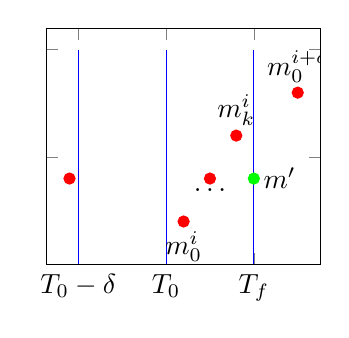
\begin{tikzpicture}
        \begin{axis}[
          % width=10cm,
          scale only axis, height=3cm,
          ymin = 0,
          yticklabels= {},
          xticklabels={$\ldots$,$t_{i-1}^N$,$T_0-\delta$,$T_0$,$T_f$},
          ]
          \addplot[ycomb,blue] coordinates {
            (20,10)
            (30,10)
            (40,10)
          }; 
          
          \addplot[only marks,mark=*,red] coordinates {
            (19,4)
            (32,2)
            (35,4)
            (38,6)
            (45,8)
          };
          
          \addplot[only marks,mark=*,green] coordinates {
            (40,4)
          };
          
          
          \node[below] at (axis cs:32,2) {$m_0^i$};
          \node[below] at (axis cs:35,4) {$\ldots$};
          \node[above] at (axis cs:38,6) {$m_k^i$};
          \node[above] at (axis cs:45,8) {$m_0^{i+\delta}$};
          \node[right] at (axis cs:40,4) {$m'$};
        \end{axis}
      \end{tikzpicture}
    \end{center}
  \end{columns}
\end{frame}


%%% Local Variables: 
%%% ispell-local-dictionary: "british"
%%% mode: latex
%%% TeX-master: "presentacio"
%%% End: 
